
\documentclass[a4paper]{article}
\usepackage{interlude}
\usepackage{pslatex}
\usepackage[T1]{fontenc}
\usepackage[utf8x]{inputenc}
\setlength\parskip{\medskipamount}
\setlength\parindent{0pt}
\usepackage{graphicx}
\usepackage{amssymb}
%\usepackage{hyperref}

\makeatletter

\providecommand{\boldsymbol}[1]{\mbox{\boldmath $#1$}}
\newcommand{\ASL}			{ASL}
\newcommand{\OSC}[1]		{\texttt{#1}}
\newcommand{\lra}			{$\leftrightarrow$}
\newcommand{\seg}[1]		{Seg(#1)}

\setlength{\parskip}{1mm}

\makeatother

\begin{document}

\title{Augmented Score Library Specification \\ v.0.52}


\author{Grame, Centre National de Création Musicale\\
{\small <research@grame.fr>} \\
\vspace{2mm}
ANR-08-CORD-010
}

\maketitle

%\vspace{3cm}
%==================================================================================================
\section{Introduction}

The Augmented Score Library [\ASL] is intended to provide \emph{augmented music score} capabilities.
An augmented music score is a graphic space that supports music scores and arbitrary graphic resources, including real-time elements, and providing time synchronization between all the score components. For the time being, it is planned to support graphic resources such as textual elements, images (jpg, gif, tiff, png, bmp) and various signal representations. Time synchronization represents the possibility to graphically synchronize the augmented score components in order to align the graphic sections of the score components that correspond to equivalent time spaces.
Time synchronization addresses an issue identified as \emph{time to graphic mapping}, which is the core of the augmented score research project. 

The ASL features are available using a standard C/C++ API or via \emph{Open Sound Control}\cite{OSC} [OSC]\footnote{http://opensoundcontrol.org/} messages. There is a direct correspondence between the OSC messages and the library API. The global design of the library is based on the well known \emph{Model View Controller} [MVC] approach.

%==================================================================================================
\section{MVC Design}

The global architecture is illustrated in figure \ref{mvc}. Modification of the model state are achieved via the library API or incoming OSC messages. The modification requests are packaged into \emph{messages} and stacked on a lock-free fifo messages stack. These operations are synchronous to the incoming OSC stream or to the library API calls. 

On a second step, messages are popped from the stack by the \texttt{IControler}, which takes in charge address decoding and message passing to the corresponding object of the model. The model is organized as a tree, similarly to an OSC message and each node of the tree carries a name that should be used by valid OSC addresses. Address decoding consists in matching each part of the OSC address with the corresponding node until the last node of the address - the target node - is identified. 
The final step of the model modification consists in applying the message to the target object: the message is actually given to the \texttt{execute} method of the object. Each object of the model implements the necessary handlers to process its set of accepted messages. 
This second step of the model modification scheme is asynchronous: it is actually processed on a regular time base.

\begin{figure}[h]
	\centering 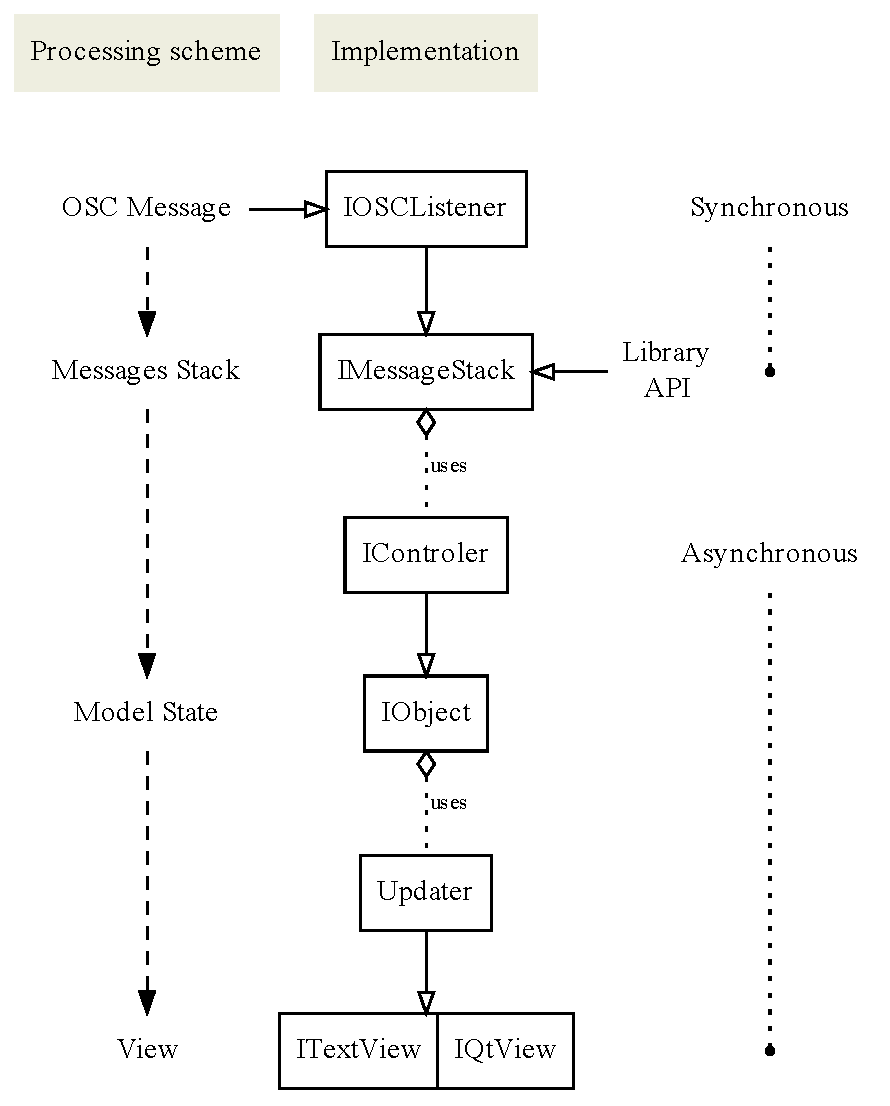
\includegraphics[width=100mm]{rsrc/mvc}
 \caption{An overview of the MVC architecture}
 \label{mvc}
\end{figure}

The final step of the processing scheme concerns the \emph{view} update. It is implemented using the \emph{visitor} design pattern \cite{DP95}. An \texttt{Updater} provides the necessary to browse the model tree and call the derived \texttt{updateTo} method only when necessary i.e. when the corresponding node is modified. An \texttt{Updater} is in charge of producing a view of the model. Two updaters are currently supported: an updater producing a textual view of the model (\texttt{ITextView}) and an updater producing a graphic view based on the Qt Framework (\texttt{IQtView}).

%==================================================================================================
\section{The Model Hierarchy}

The figure \ref{model} presents the model hierarchy. It is made of 
\begin{itemize}
\item static objects: predefined objects that can't be created or deleted by client applications.
\item dynamic objects: objects created by client applications.
\item virtual objects: objects automatically embedded into another object.
\end{itemize}

\begin{figure}[h]
	\centering 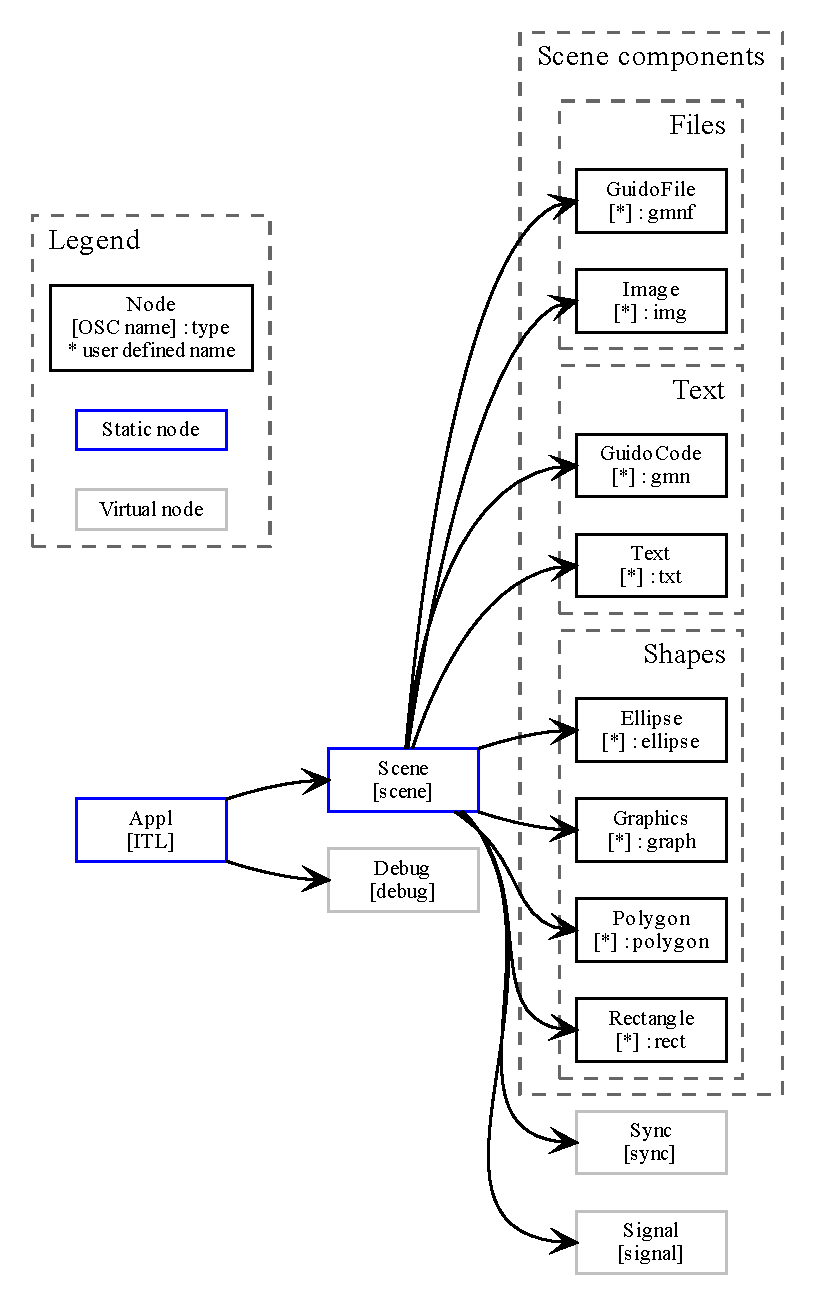
\includegraphics[width=90mm]{rsrc/model}
 \caption{A non-exhaustive view of model hierarchy}
 \label{model}
\end{figure}

Objects of the model are grouped by category:
\begin{itemize}
\item \emph{Files} corresponds to file based components: an image file or a Guido GMN file. 
\item \emph{Text} corresponds to textual components not based on a file.
\item \emph{Shapes} corresponds to vectorial graphics (ellipse, rectangle, polygon) and to a component named \emph{Graphics} that takes a signal as input to produce a graphic representation of this signal.
\end{itemize}

Each object of the model has a name used as a identifier: static and virtual objects carry predefined names, all the other objects names are defined by the client application. A name must be unique for a given hierarchy level.
The object's type mentioned in figure \ref{model} is detailed in the OSC messages documentation.

%==================================================================================================
\section{The Update Process}

The update process is actually composed of several steps (see figure \ref{update}):
\begin{itemize}
\item a first step consists in setting the model data according to the incoming messages
\item the second step may be viewed as the partial integration of the view into the model: this step is intended to compute all the information necessary to process the next step, which is basically the graphic segmentation of an object and, depending on the object type, the necessary segmentations and mappings to go from the graphic to the time space \cite{fober10a}.
\item the third step computes the mapping that goes from an object local space segmentation to the corresponding graphic segments.
\item the last step draw the objects according to the relations computed at the preceding step.
\end{itemize}

\begin{figure}[h]
	\centering 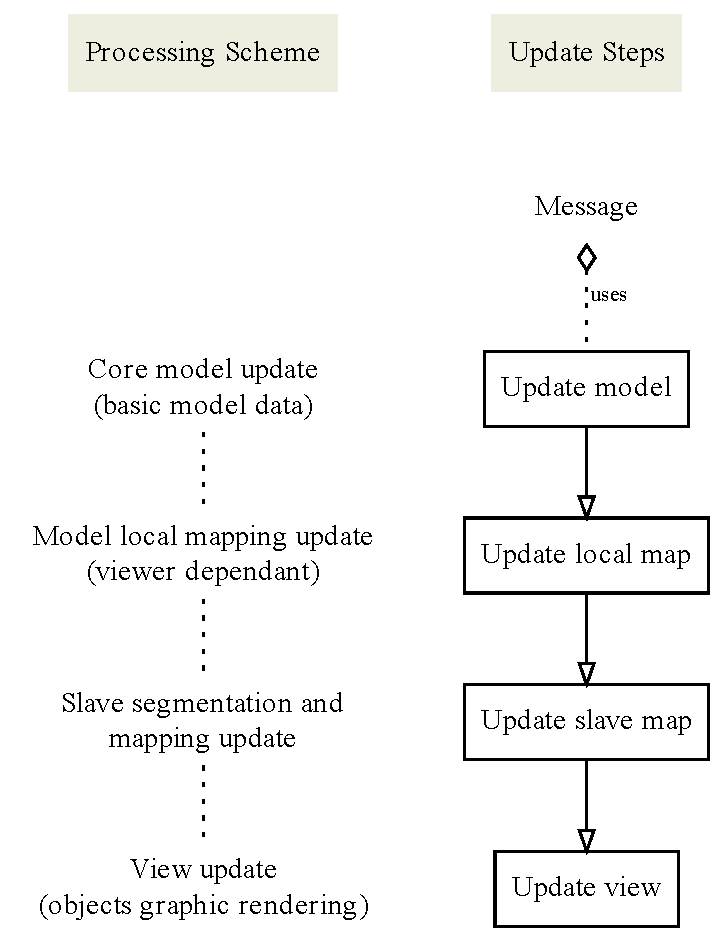
\includegraphics[width=80mm]{rsrc/update}
 \caption{Details of the update process}
 \label{update}
\end{figure}

All these steps are detailed in the next sections.


%==================================================================================================
\subsection{Core model update}
to do... describe the messages processing scheme (handlers etc...)


%==================================================================================================
\subsection{Local mapping update of the model}

Table \ref{maptable} lists the segmentations and mappings used by the different component types. Mappings are indicated using arrows (\lra). Note that the arrows link segments of different types (the \emph{segment} qualifier is omitted). Segmentations and mappings in  \textit{italic} are automatically computed by the system, those in \textbf{bold} are to be provided externally.

\begin{table}[htdp]
\begin{center}
\begin{tabular}{|r|l|}
\hline
type & segmentations and mappings required \\
\hline
text		& \textit{graphic} \lra\ \textbf{text  \lra\ time} \\
score		& \textit{graphic \lra\ wrapped time} \lra\ \textit{time} \\
image		& \textit{graphic} \lra\ \textbf{pixel \lra\ time} \\
vectorial graphic	&  \textit{graphic} \lra\ \textbf{vectorial \lra\ time} \\
signal		&  \textit{graphic} \lra\ \textbf{frame \lra\ time} \\
\hline
\end{tabular}
\end{center}
\caption{Segmentations and mappings for each component type}
\label{maptable}
\end{table}

The second step of the update process is in charge of computing the segmentations and mappings in \textit{italic}.
The computation is illustrated in figure \ref{localmap}, blue arrows denotes mappings to be computed by the local mapping update.
\begin{figure}[h]
	\centering 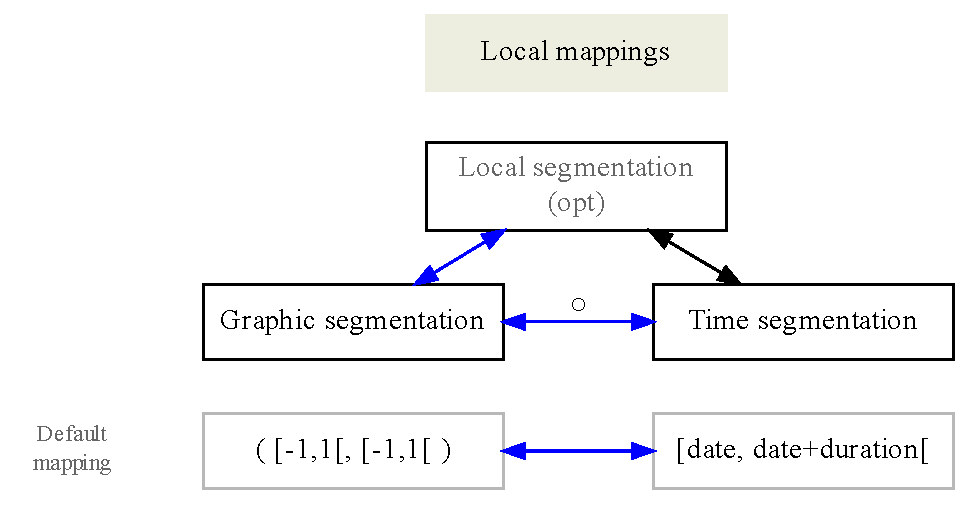
\includegraphics[width=100mm]{rsrc/localmappings}
 \caption{Local mappings computation: arrows in blue indicate the computations.}
 \label{localmap}
\end{figure}

%====================================
\subsubsection{Events that trigger the local mapping update}
A local mapping needs to be updated when:
\begin{itemize}
\item the corresponding mapping provided externally has changed
\item the object data has changed
\item the object duration has changed and the duration is used for default mapping
\end{itemize}


%==================================================================================================
\subsection{Slave segmentation and mapping update}

This step is intended to prepare the objects graphic rendering (update process, last step) and to make graphic synchronization transparent for the rendering process. The basic principle is to compute a mapping from an object local graphic space to its master graphic space. 

Details of the mapping computation according to an object relations is given below. For the next sub-sections, we assume that the target object $O$ of the update process has the following properties:
\vspace{-2mm}
\begin{itemize}
\item it holds a time space segmentation $\seg{O_{t}}$
\item it holds a graphic space segmentation $\seg{O_{g}}$
\item it holds a mapping between graphic and time space segmentations $R_{O_{g<->t}}$
\end{itemize}

%Note that when no mapping has been explicitely set for an object, implicit segmentations and mapping are computed such as:
%\vspace{-2mm}
%\begin{itemize}
%\item $\seg{O_{t}} = [date, duration[$
%\item $\seg{O_{l}}$ is a single segment containing the whole object ressource.
%\item $R_{O_{l<->t}}$ associates the single time segment and the single local segment.
%\end{itemize}

Next and when the target object has a slave relation with a master object $M$, we assume that $M$ has the following properties :
\vspace{-2mm}
\begin{itemize}
\item it holds a time segmentation $\seg{M_{t}}$
\item it holds a graphic space segmentation $\seg{M_{g}}$
\item it holds a mapping between time and graphic spaces segmentations $R_{M_{t<->g}}$
\end{itemize}
Note that the graphic space segmentation is expressed in the owner object local coordinates.

%====================================
\subsubsection{Mapping an object without synchronization}
The update process has nothing to do. No mapping is used and the $x$, $y$ and $scale$ properties are left unchanged.

%====================================
\subsubsection{Mapping a synchronized object without time stretching}
The update process don't compute any mapping from local to graphic space but modifies the object $x$ and $y$ coordinates:
\vspace{-2mm}
\begin{itemize}
\item it retrieves the segment $M_{date}$ containing the object $date$ from $\seg{M_{t}}$
\item it gets the corresponding graphic segment $M_{g} \in \seg{M_{g}}$ from $R_{M_{t<->g}}$
\item and finally sets the object $x$ to the corresponding position in $M_{g}$, obtained by linear interpolation and set $y$ to the center of $M_{g}.y$ axis.
\end{itemize}
Note that the slave object coordinates are expressed in its master coordinates space.

Depending on the optional vertical stretch mode, the object $scale$ property is computed as the ratio between $M_{g}.y$ interval size and the object $height$.

%====================================
\subsubsection{Mapping a synchronized object with time stretching}
The update process computes the mapping $R_{O_{g}<->M_{g}} = R_{O_{g<->t}} \circ\ R_{M_{t<->g}}$\\
Note that it may involve the computation of \emph{virtual} segments since $\seg{O_{t}}$ and $\seg{M_{t}}$ don't necessary match. The virtual segments computation makes use of linear interpolation. \\
%The object $x$ and $y$ position are set as described above but using the first graphic segment $M_{g0}$. \\
%Depending on the stretch mode, the object $scale$ property is computed as the ratio between $M_{g0}.y$ interval size and the object $height$.

The computation is illustrated in figure \ref{slavemap}, blue arrows denotes mappings to be computed by the slave mapping update. Note that it involves a virtual mapping since the slave and master segmentations don't necessary match.

\begin{figure}[h]
	\centering 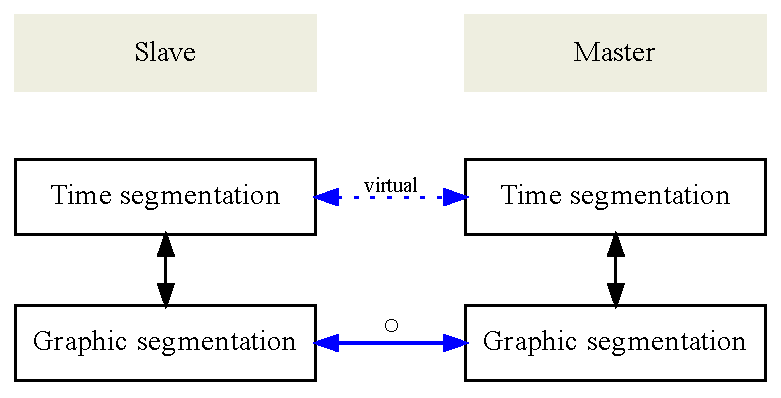
\includegraphics[width=90mm]{rsrc/mappings}
 \caption{The slave mapping computation: arrows in blue indicate the computations.}
 \label{slavemap}
\end{figure}

%====================================
\subsubsection{Mappings translation}
The $date$ of an object is used to translate the time segmentation of a slave object. The translation consists in shifting every time segment from the $date$ value. 
%Depending on the synchronzation mode (to be defined), the translation could be static (stored as a new Time segmentation) or dynamic (computed by the slave segmentation and mapping update).

%====================================
\subsubsection{Events that trigger the slave mapping update}

The slave to master mapping needs to be updated when:
\begin{itemize}
\item the slave date has changed
\item the slave or the master local mapping has been updated
\item the synchronization mode has changed 
\end{itemize}


%==================================================================================================
\subsection{View update}
The view update consists in actual graphic rendering of an object. We make a distinction between the rendering of objects holding a mapping from local space to graphic space and those that don't:

\begin{itemize}
\item Rendering objects without mapping: the object is actually drawn using its current $x$, $y$ and $scale$ properties.
\item Rendering objects with mapping: for each associated segments $O_{l}$ and  $M_{g}$ taken from $R_{O_{l<->g}}$:
\begin{itemize}
	\item depending on the stretch mode, computes a $scale$ as the ratio between $M_{g}.y$ interval size and the object $height$.
	\item draw the segment $O_{l}$ at the $x$ and $y$ coordinates taken from $M_{g}$ and using the object $scale$.
\end{itemize}

\end{itemize}



\bibliographystyle{unsrt}
\bibliography{specification}

\end{document}
